\section{Performance}
\label{sec:performance}

We study the separation of the $\dihiggs$ signal from the $\ttbar$ background,
achieved by the LR $P(\vecy)$ given by Eq.~(\ref{eq:memLR}),
using samples of signal and background events produced by Monte Carlo (MC) simulation.
The samples are simulated at LO and at NLO accuracy in pQCD
and are analyzed at MC-truth as well as at detector level.
The LO and NLO $\dihiggs$ signal samples each contain about three hundred thousand events
and the LO and NLO $\ttbar$ background samples each contain about five million events.
All samples simulated at LO accuracy in pQCD are produced with the program $\textsc{MadGraph\_aMCatNLO}$ $2.2.2$,
while the samples simulated at NLO accuracy in pQCD are produced using the program $\textsc{POWHEG}$ $v2$~\cite{POWHEG1,POWHEG2,POWHEG3,POWHEGTTBAR1,POWHEGTTBAR2,POWHEGHH1,POWHEGHH2}.
The \textrm{NNPDF3.0} LO set of PDF is used for the simulation of the LO samples and the \textrm{NNPDF3.0} NLO set for the NLO samples~\cite{NNPDF1,NNPDF2,NNPDF3}.
Parton shower and hadronization processes are modeled using the program $\textsc{PYTHIA}$ $v8.2$~\cite{Sjostrand:2014zea} with the tune \textrm{CP5}~\cite{Sirunyan:2019dfx}.
All events are generated for proton-proton collisions at $\sqrt{s} = 13$~\TeV center-of-mass energy.
Events in which the electrons or muons originate from $\Pgt$ lepton decays,
\ie from the decay chains $\PW^{+} \to \Pgt^{+}\Pnu_{\Pgt} \to \Plepton^{+}\Pnu_{\Plepton}\APnu_{\Pgt}\Pnu_{\Pgt}$ or 
$\PW^{-} \to \Pgt^{-}\APnu_{\Pgt} \to \Plepton^{-}\APnu_{\Plepton}\Pnu_{\Pgt}\APnu_{\Pgt}$, are discarded.
Detector effects are simulated using the $\textsc{DELPHES}$ fast-simulation package~\cite{deFavereau:2013fsa} with the card for the CMS detector.
On average forty inelastic proton-proton interactions (pileup) are added to each simulated event
in order to simulate the data-taking conditions during Run $2$ of the LHC.

Jets are reconstructed using the anti-$\kt$ algorithm~\cite{Cacciari:2008gp, Cacciari:2011ma} with a distance parameter of $0.4$.
We produce two separate collections of jets for studying the performance of the MEM at MC-truth and at detector level,
using either all stable generator-level particles or the detector-level particle-flow objects created by $\textsc{DELPHES}$ as input to the jet reconstruction.
We refer to the first collection as generator-level and to the second as detector-level jets.
The generator-level jets exclude the particles from pileup.
The energy of jets reconstructed at detector level is corrected for pileup effects using the method described in Refs.~\cite{Cacciari:2008gn, Cacciari:2007fd}
and calibrated as function of jet $\pT$ and $\eta$, where $\eta = -\ln\tan(\theta/2)$ denotes the pseudorapidity of the jet.
The calibration is performed in two stages. 
In the first stage, the energy of detector-level jets is calibrated to match the energy of generator-level jets,
while in the second stage, the energy of generator-level jets is calibrated to match the energy of the bottom quarks that result from $\PHiggs$ boson or top quark decays at parton level.
The first stage of the jet energy calibration is applied to all detector-level jets, 
while the second stage is applied to the generator-level jets and to those detector-level jets that are tagged, on detector level, as originating from the hadronization of a bottom quark.
We refer to the latter jets as $\Pbottom$-jets.

The simulated $\dihiggs$ signal and $\ttbar$ background events considered in this section are required to pass event selection criteria
similar to the analysis of $\dihiggs$ production in the decay channel $\Pbottom\APbottom\PW\PW\virt$ performed by the CMS collaboration in LHC Run $2$~\cite{HIG-17-006}.
The events are required to contain two electrons or muons and two $\Pbottom$-jets.
The leptons must be within the region $\abs{\eta} < 2.5$ if they are electrons and $\abs{\eta} < 2.4$ if they are muons, and are required to be isolated.
Their isolation is computed by summing the $\pT$ of detector-level particle-flow objects that are within a cone of size
$\delta R = \sqrt{(\delta\eta)^{2} + (\delta\phi)^{2}} = 0.5$ around the lepton direction, excluding the lepton itself.
The sum is corrected for the contribution of particles from pileup using the method described in Refs.~\cite{Cacciari:2008gn, Cacciari:2007fd}.
Electrons and muons are considered isolated if the pileup-corrected sum amounts to less than $0.10$ times the $\pT$ of the lepton.
The lepton of higher $\pT$ is required to have $\pT > 25$~\GeV and the lepton of lower $\pT$ must have $\pT > 15$~\GeV.
The $\pT$ thresholds applied to the leptons are motivated by trigger requirements.
The $\Pbottom$-jets are required to satisfy the conditions $\pT > 25$~\GeV and $\abs{\eta} < 2.4$ and to be both tagged as $\Pbottom$-jets on detector level.
The $\Pbottom$-tagging criteria implemented in the $\textsc{DELPHES}$ card for the CMS detector
corresponds to the XXX working-point of the XXX $\Pbottom$-tagging algorithm published in Ref.~\cite{}.
Events containing more than two $\Pbottom$-tagged jets of $\pT > 25$~\GeV and $\abs{\eta} < 2.4$ are vetoed.
The latter condition rejects a negligible fraction of events, amounting to $X.X\%$ of the $\dihiggs$ signal and $X.X\%$ of the $\ttbar$ background,
and avoids ambiguities in choosing the pair of $\Pbottom$-jets 
when computing the PDs $w_{0}(\vecy)$ and $w_{1}(\vecy)$ according to Eqs.~\ref{eq:mem_signal} and~\ref{eq:mem_background}.
The selection criteria are applied either to generator-level leptons and jets (when analyzing simulated events at MC-truth level) 
or to the detector-level leptons and jets created by $\textsc{DELPHES}$ (when analyzing simulated events at detector level).
In case the selection criteria are applied at MC-truth level,
the $\pT > 25$~\GeV and $\abs{\eta} < 2.4$ requirements are applied on the generator-level jets that originate from the hadronization of the bottom quarks 
produced in the $\PHiggs$ boson or top quark decays and no detector-level $\Pbottom$-tagging criteria are applied.

Fig.~\ref{fig:mbb} shows the distribution in $\mbb$, the mass of the two $\Pbottom$-tagged jets at detector level, 
in $\dihiggs$ signal and $\ttbar$ background events that pass the selection criteria described in the previous paragraph.
Only events in which both detector-level jets are matched, within a cone of size $\delta R = 0.3$, 
to bottom quarks that originate from either $\PHiggs$ boson or from top quark decays, are shown in the figure.
According to the $\textsc{DELPHES}$ simulation, 
$XX.X\%$ of $\dihiggs$ and $XX.X\%$ of $\ttbar$ events that pass the selection criteria described in the previous paragraph fulfill this matching condition,
\ie in $X.X\%$ of selected $\dihiggs$ and $X.X\%$ of selected $\ttbar$ events one of the bottom quarks is not reconstructed as $\Pbottom$-jet at detector level
and a light quark or gluon jet is misidentified as $\Pbottom$-jet instead.
The figure shows that the jet calibration shifts the peak of the $\mbb$ distribution by about $20\%$.
After calibration, the $\mbb$ distribution in $\dihiggs$ signal events peaks close to $125$~\GeV.
The calibration also reduces the relative width, defined as the root mean square divided by the mean, of the $\mbb$ distribution in $\dihiggs$ signal events by about $20\%$.

\begin{figure}
\ifx\ver\verPreprint
\setlength{\unitlength}{1mm}
\begin{center}
\begin{picture}(160,67)(0,0)
\put(-1.0, 1.0){\mbox{\includegraphics*[height=66mm]
 {plots/mbb_calibrated_vs_uncalibrated_signal.pdf}}}
\put(80.0, 0.0){\mbox{\includegraphics*[height=67mm]
 {plots/mbb_calibrated_vs_uncalibrated_background.pdf}}}
\end{picture}
\end{center}
\fi
\ifx\ver\verPAPER
\centering
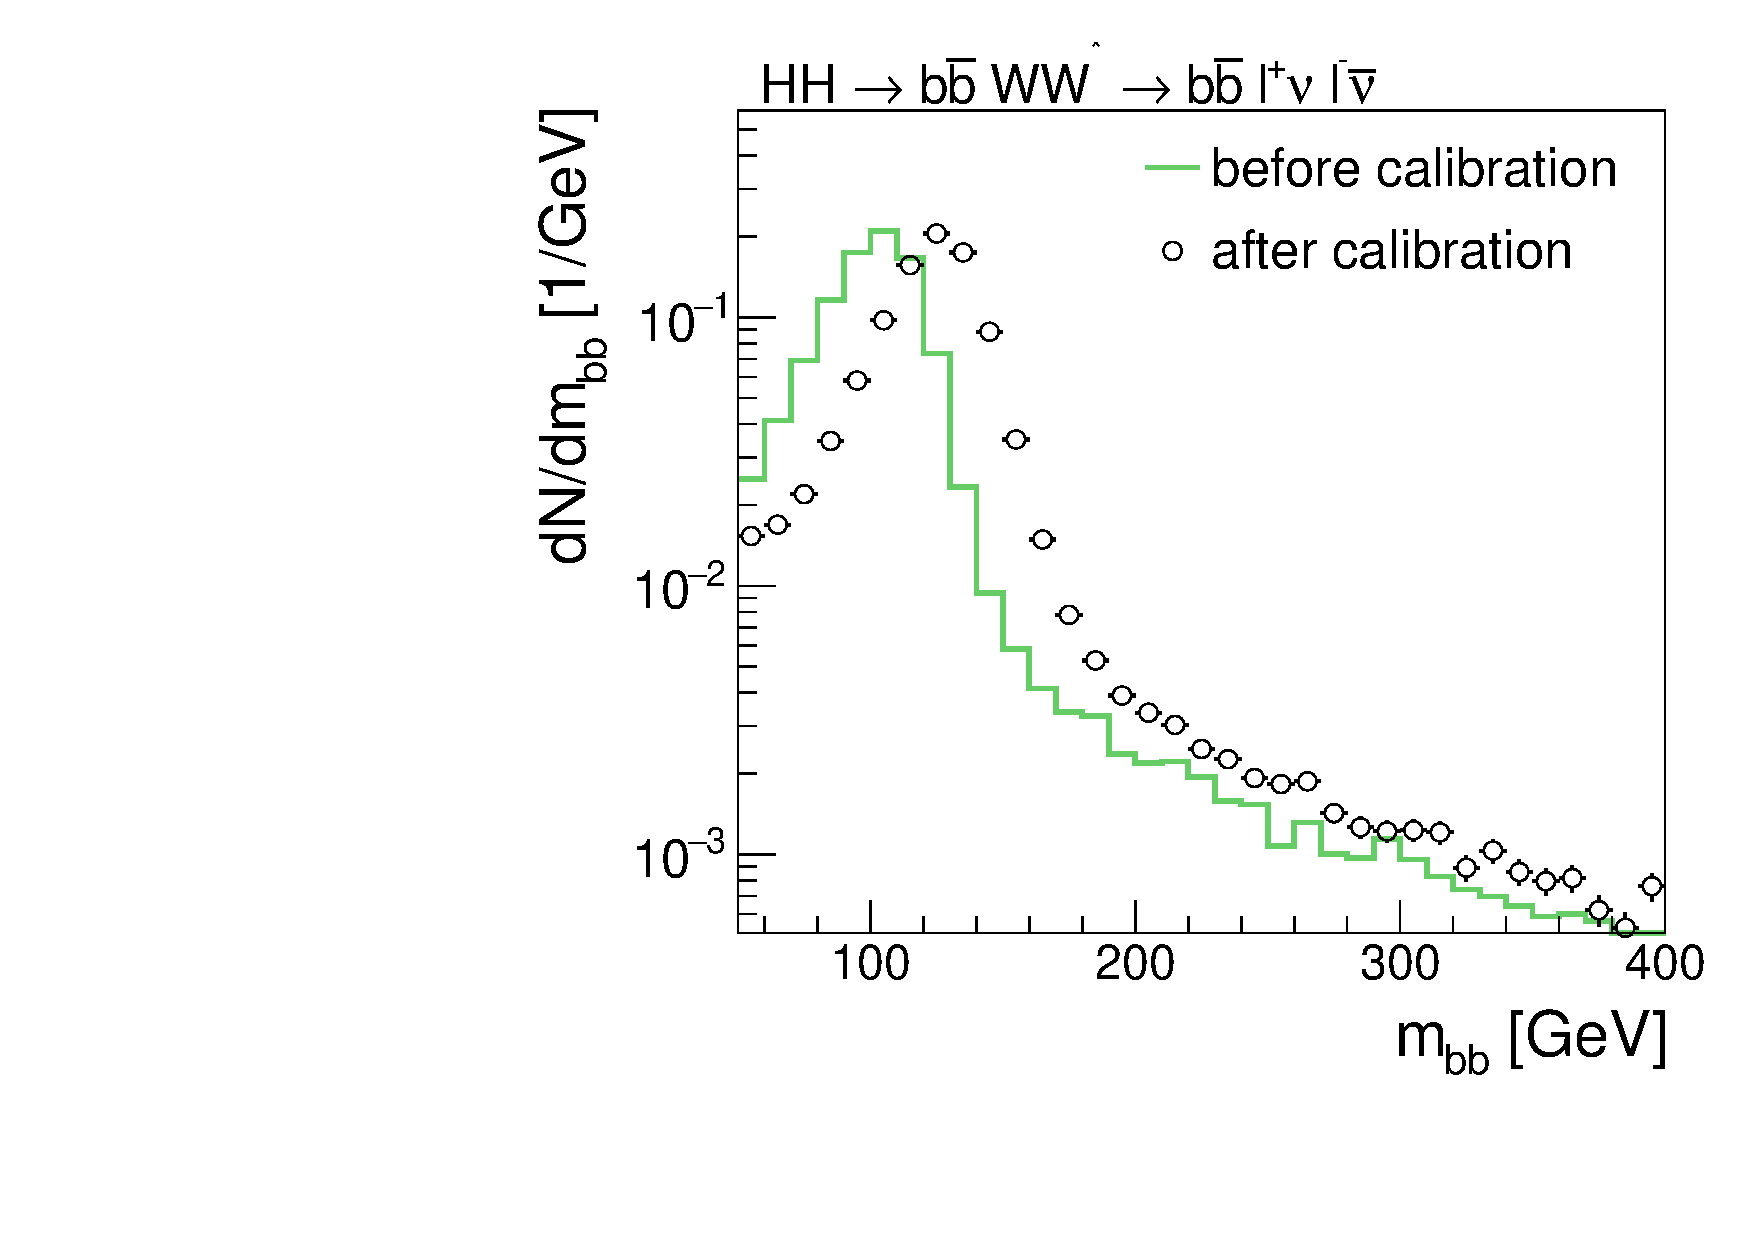
\includegraphics[width=0.48\textwidth]{plots/mbb_calibrated_vs_uncalibrated_signal.pdf}
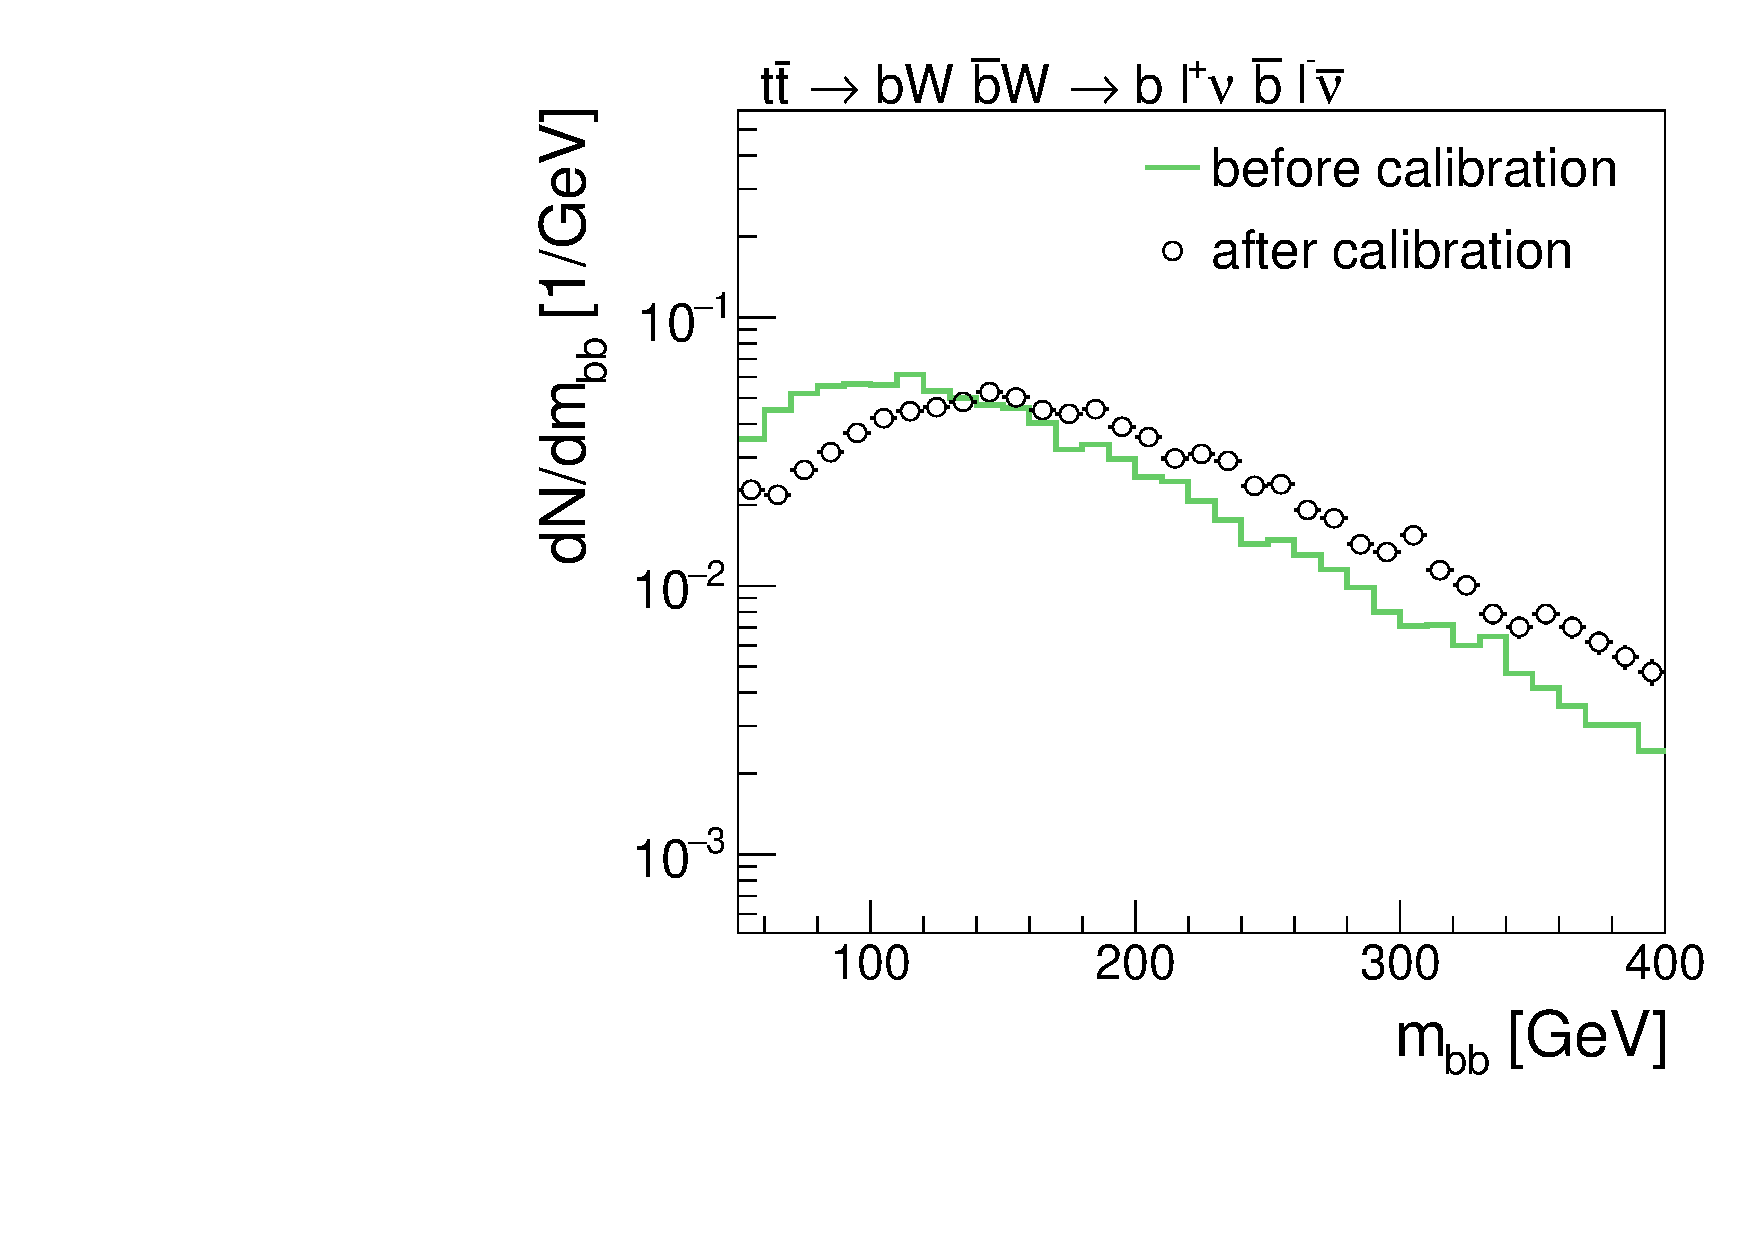
\includegraphics[width=0.48\textwidth]{plots/mbb_calibrated_vs_uncalibrated_background.pdf}
\fi
\caption{
  Distribution in $\mbb$, the mass of the two detector-level jets that are tagged as $\Pbottom$-jets,
  in $\dihiggs$ signal (left) and $\ttbar$ background (right) events before and after the jet energy calibration is applied.
}
\label{fig:mbb}
\end{figure}

Before we can compute the PDs $w_{0}(\vecy)$ and $w_{1}(\vecy)$ according to Eqs.~\ref{eq:mem_signal} and~\ref{eq:mem_background},
we need to determine the TF for the energy of $\Pbottom$-jets and for the transverse momentum components of the hadronic recoil
such that the TF match the experimental resolutions in the $\textsc{DELPHES}$ simulation.
We model the experimental resolution on the energy of $\Pbottom$-jets using a normal distribution:
\begin{linenowrapper}
\begin{equation}
W(E|\Ehat) = \frac{1}{\sqrt{2 \pi \sigma_{\Pbottom}^{2}}} \, e^{-\frac{(\pT - \pThat)^{2}}{2 \, \sigma_{\Pbottom}^{2}}} \, ,
\label{eq:resolution_b}
\end{equation}
\end{linenowrapper}
where $\pT = E \, \sin\theta$, $\pThat = \Ehat \, \sin\theta$, and $\theta$ refers to the polar angle of the jet.
The standard deviation $\sigma_{\Pbottom}$ depends on the jet energy and $\theta$.
We make the ansatz $\sigma_{\Pbottom} = k \cdot \sqrt{\Ehat \, \sin\theta}$ and determine the constant of proportionality $k$ such that it fits
the resolution on the energy of $\Pbottom$-jets in the $\textsc{DELPHES}$ simulation, yielding $k = 100\%$.
Our model for the jet energy resolution agrees with the resolution measured by the CMS collaboration during LHC Run $2$ that is shown in Fig.~3 of Ref.~\cite{JME-18-001}.
Our assumption that the polar angle $\theta$ of the jet is measured with negligible experimental resolution (\cf Section~\ref{sec:appendix_TF} of the appendix)
is justified by Fig.~5 of Ref.~\cite{JME-18-001}, which shows that the resolution on $\theta$ amounts to about $0.02$ radians for jets of $\pT = 25$~\GeV and decreases for jets of higher $\pT$.
The hadronic recoil $\rho$ is not directly available in the $\textsc{DELPHES}$ simulation.
To determine the resolution on $\rho$, we compute the transverse momentum components of the hadronic recoil by means of Eq.~\ref{eq:hadRecoil_true} at MC-truth
and by means of Eq.~\ref{eq:hadRecoil} at detector level.
The resolutions on $\pX^{\rho}$ and $\pY^{\rho}$ amount to $XX.X$~\GeV for the $\dihiggs$ signal and to $XX.X$~\GeV for the $\ttbar$ background.
The resolution on the energy of $\Pbottom$-jets is small compared to the resolution on the hadronic recoil,
which means that the resolution on the latter is dominated by the resolution on the $\vecMET$.
This allows us to compare the resolutions on $\pX^{\rho}$ and $\pY^{\rho}$ in the $\textsc{DELPHES}$ simulation to published $\vecMET$ resolutions during LHC Run $2$.
The $\vecMET$ resolution for simulated $\ttbar$ events in the ATLAS detector is shown in Fig.~9 of Ref.~\cite{ATLAS:2018txj} and amounts to $25$-$30$~\GeV,
similar to what we find with $\textsc{DELPHES}$ for the CMS detector (we did not find numbers published by CMS for the $\vecMET$ resolution in $\ttbar$ events during LHC Run $2$).
We assume that the resolutions on $\pX^{\rho}$ and $\pY^{\rho}$ are uncorrelated and the same for signal and background events.
Thus, we use:
\begin{linenowrapper}
\begin{equation}
V = \sigma_{\rho}^{2} \cdot I_{2} 
\label{eq:resolution_rho}
\end{equation}
\end{linenowrapper}
with $\sigma_{\rho} = XX.X$~\GeV for when computing the PDs $w_{0}(\vecy)$ and $w_{1}(\vecy)$ for $\dihiggs$ signal and $\ttbar$ background events.

With these TF, we can proceed to compute the PDs $w_{0}(\vecy)$ and $w_{1}(\vecy)$.
Distributions in $w_{0}(\vecy)$ and $w_{1}(\vecy)$ for $\dihiggs$ signal and $\ttbar$ background events are shown in Fig.~\ref{fig:probS_and_probB}.
The axis of abscissae is drawn in logarithmic scale to better visualize small values of the PDs.
The PDs are computed at MC-truth and at detector level.
When computing the PDs at MC-truth level, 
we set the ``measured'' momenta of electrons and muons to their generator-level values, the ``measured'' momenta of the $\Pbottom$-jets to the momenta of the corresponding parton-level bottom quarks,
and the ``measured'' transverse momentum components of the hadronic recoil to their true values $\pXhat^{\rho}$ and $\pYhat^{\rho}$.
The latter are computed according to Eq.~\ref{eq:hadRecoil_true}.
We also demand that both $\Pbottom$-jets are matched, within a cone of size $\delta R = 0.3$,
to bottom quarks that originate from either $\PHiggs$ boson or from top quark decays when we compute the PDs at MC-truth level.
The same TF, described in the previous paragraph, are used when computing the PDs $w_{0}(\vecy)$ and $w_{1}(\vecy)$ at MC-truth and at detector level.
The distributions in the PDs for the ``correct'' hypothesis ($w_{0}(\vecy)$ for signal and $w_{1}(\vecy)$ for background events)
peak close to one and fall rapidly towards smaller values, while the distributions in the PDs for the ``wrong'' hypothesis
($w_{1}(\vecy)$ for signal and $w_{0}(\vecy)$ for background events)
exhibit more pronounced tails towards small values.
Interestingly, the distributions in the PDs for the wrong hypothesis change only by a small amount between MC-truth and detector level.
The main effect of the experimental resolutions on the energy of $\Pbottom$-jets and on the transverse momentum of the hadronic recoil
as well as of the misidentification of light quark or gluon jets as $\Pbottom$-jets is to increase the tail towards small values for the distributions in the PDs for the correct hypothesis.

\begin{figure}
\ifx\ver\verPreprint
\setlength{\unitlength}{1mm}
\begin{center}
\begin{picture}(160,144)(0,0)
\put(-1.0, 78.0){\mbox{\includegraphics*[height=66mm]
 {plots/effectOfFakes_2histograms_probS_signal.pdf}}}
\put(80.0, 78.0){\mbox{\includegraphics*[height=66mm]
 {plots/effectOfFakes_2histograms_probS_background.pdf}}}
\put(-1.0, 0.0){\mbox{\includegraphics*[height=66mm]
 {plots/effectOfFakes_2histograms_probB_signal.pdf}}}
\put(80.0, 0.0){\mbox{\includegraphics*[height=66mm]
 {plots/effectOfFakes_2histograms_probB_background.pdf}}}
\end{picture}
\end{center}
\fi
\ifx\ver\verPAPER
\centering
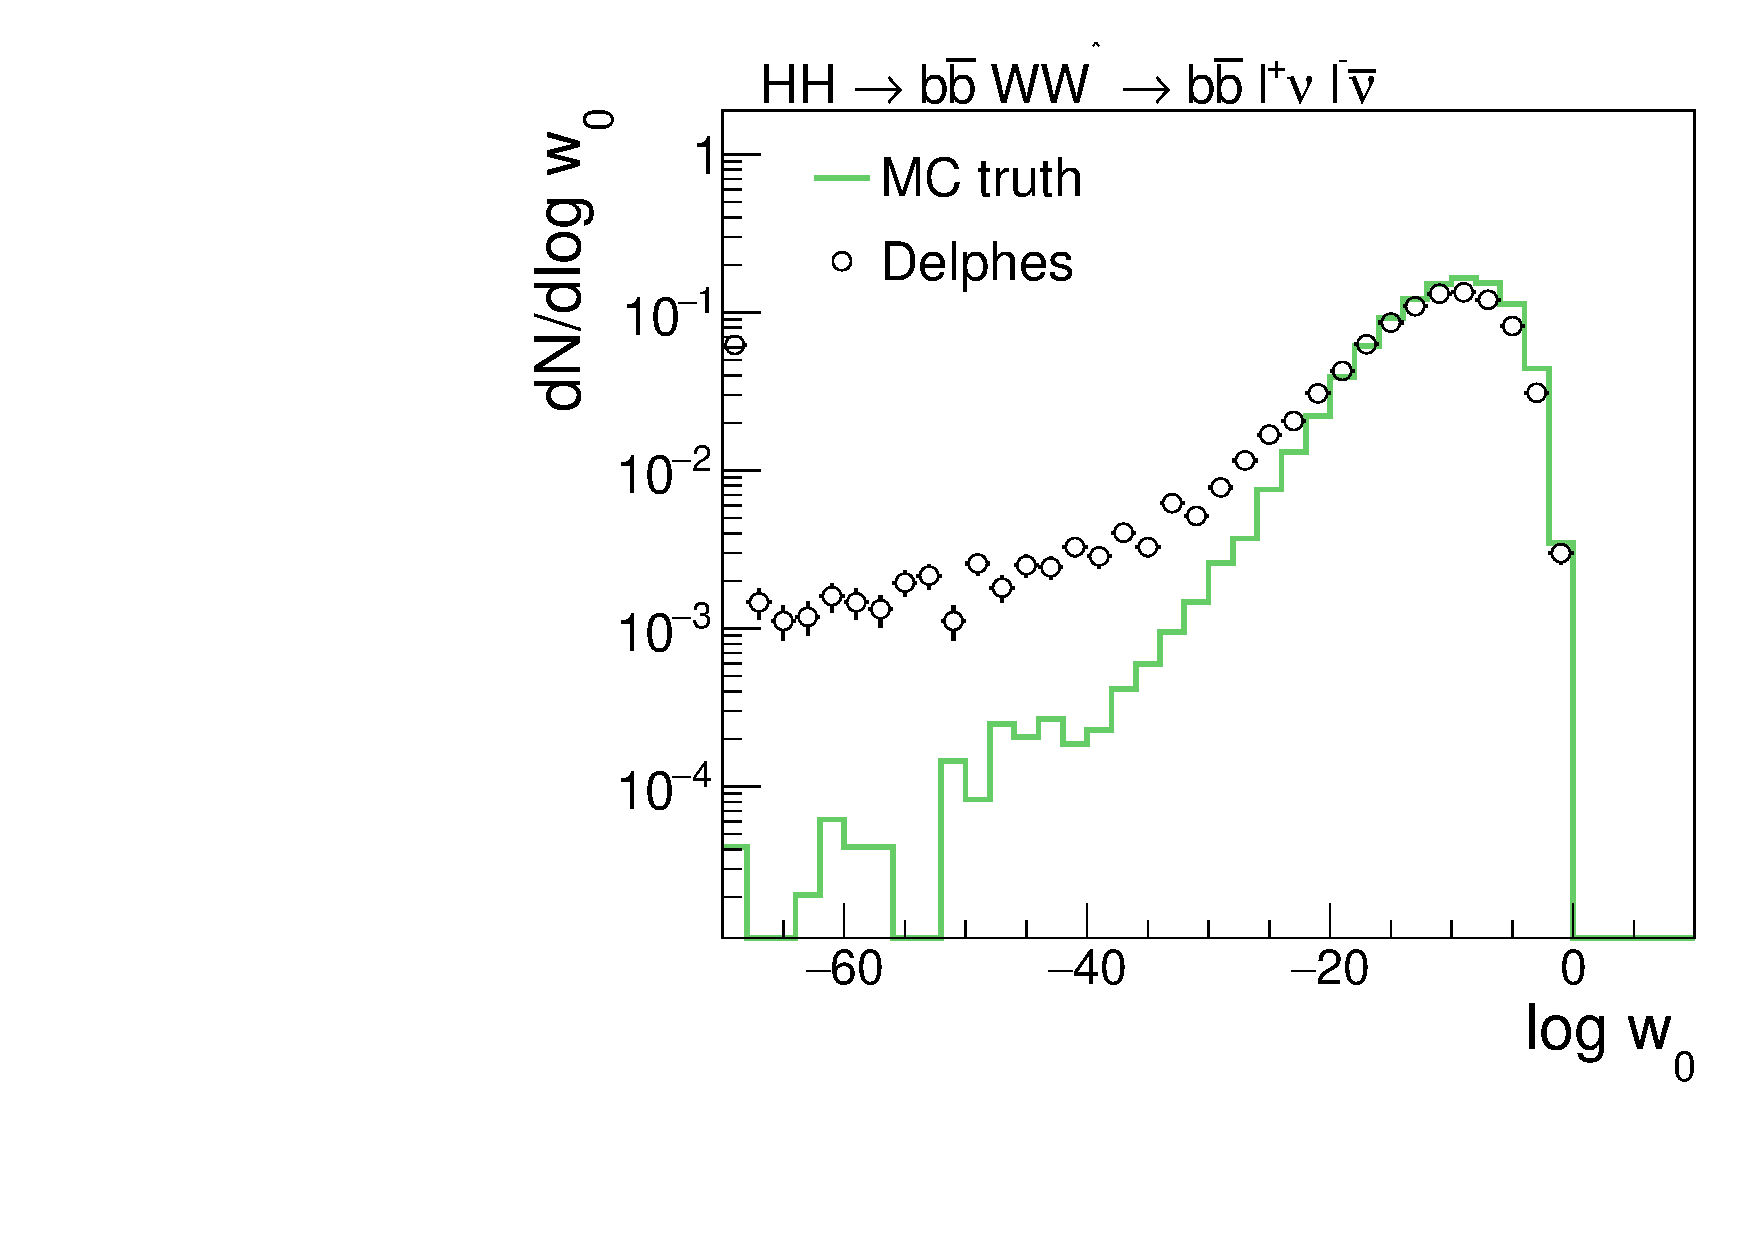
\includegraphics[width=0.48\textwidth]{plots/makePlotsForPaper_delphes_vs_mctruth_probS_signal.pdf}
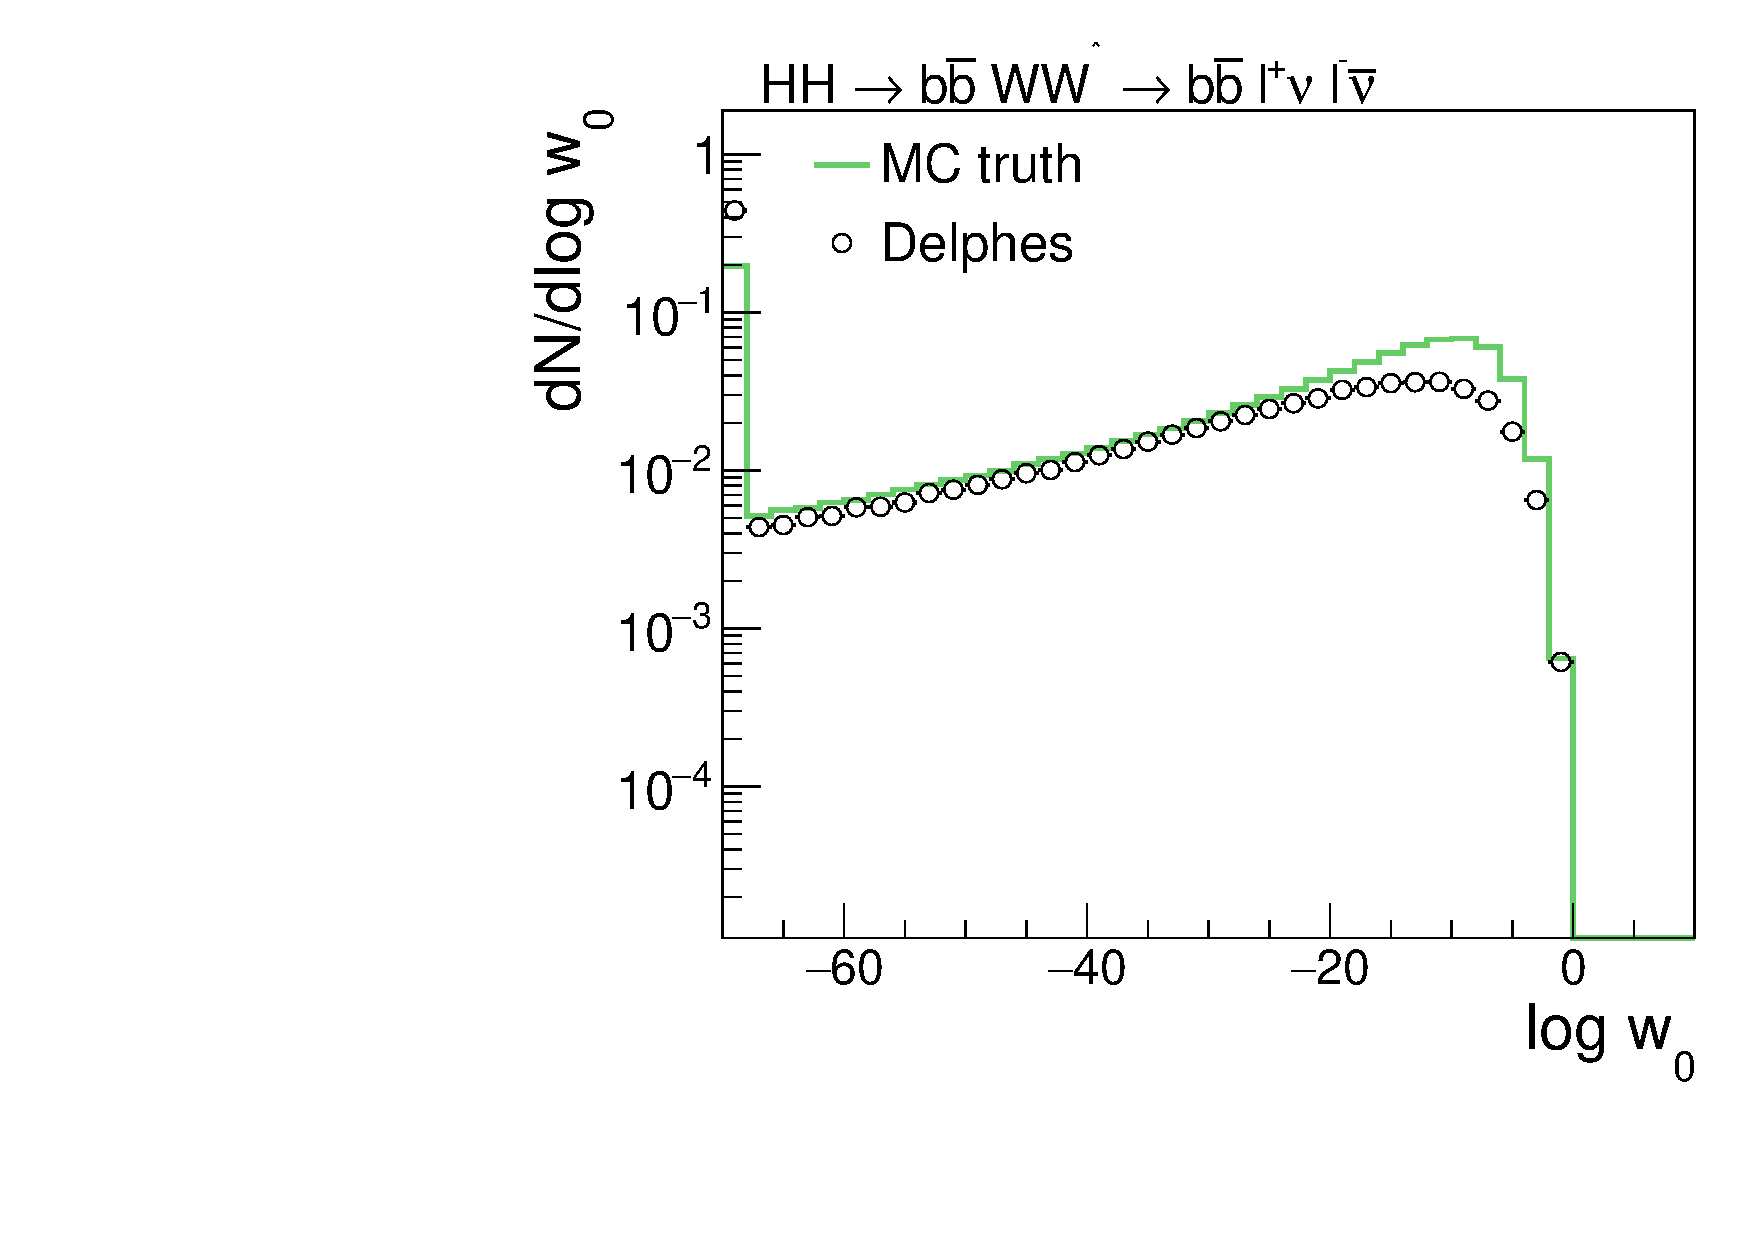
\includegraphics[width=0.48\textwidth]{plots/makePlotsForPaper_delphes_vs_mctruth_probS_background.pdf}
\hspace{0.04\textwidth}
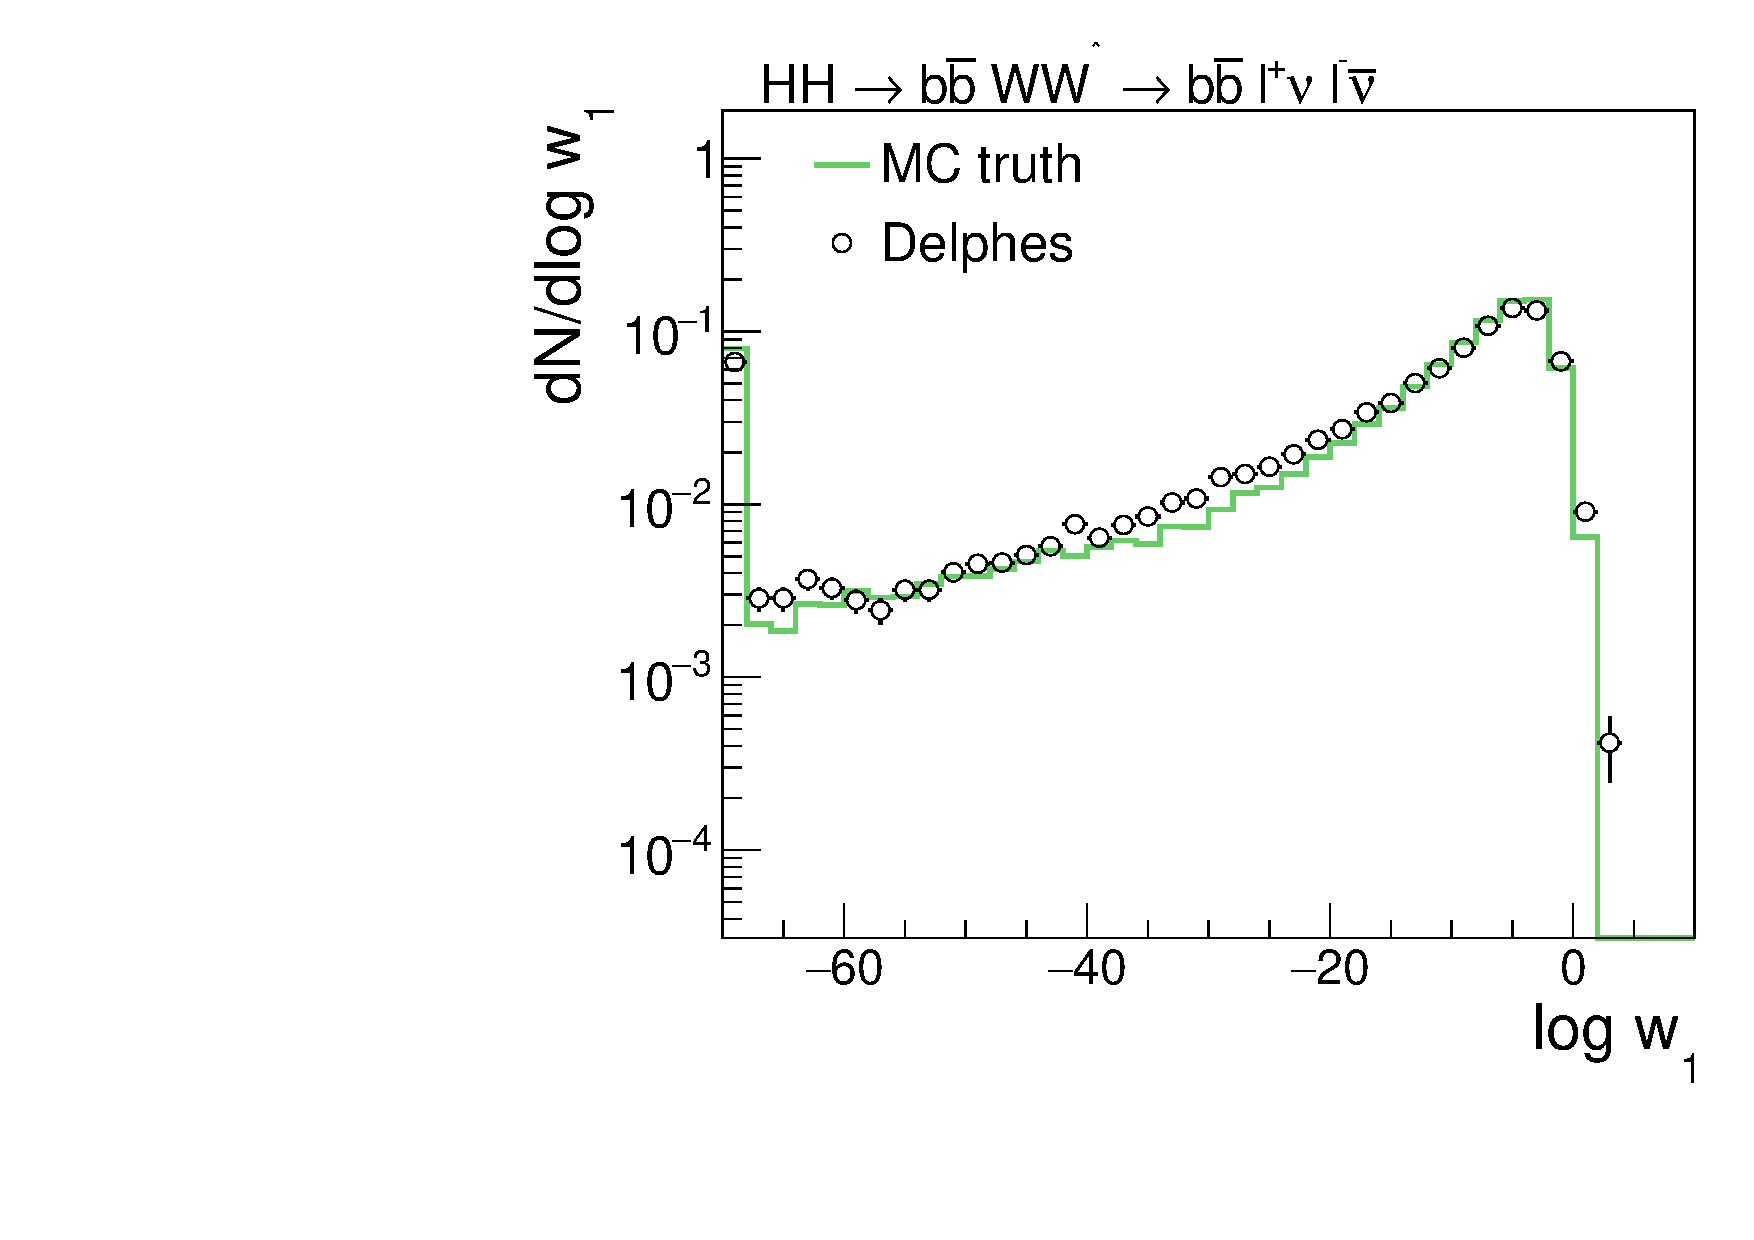
\includegraphics[width=0.48\textwidth]{plots/makePlotsForPaper_delphes_vs_mctruth_probB_signal.pdf}
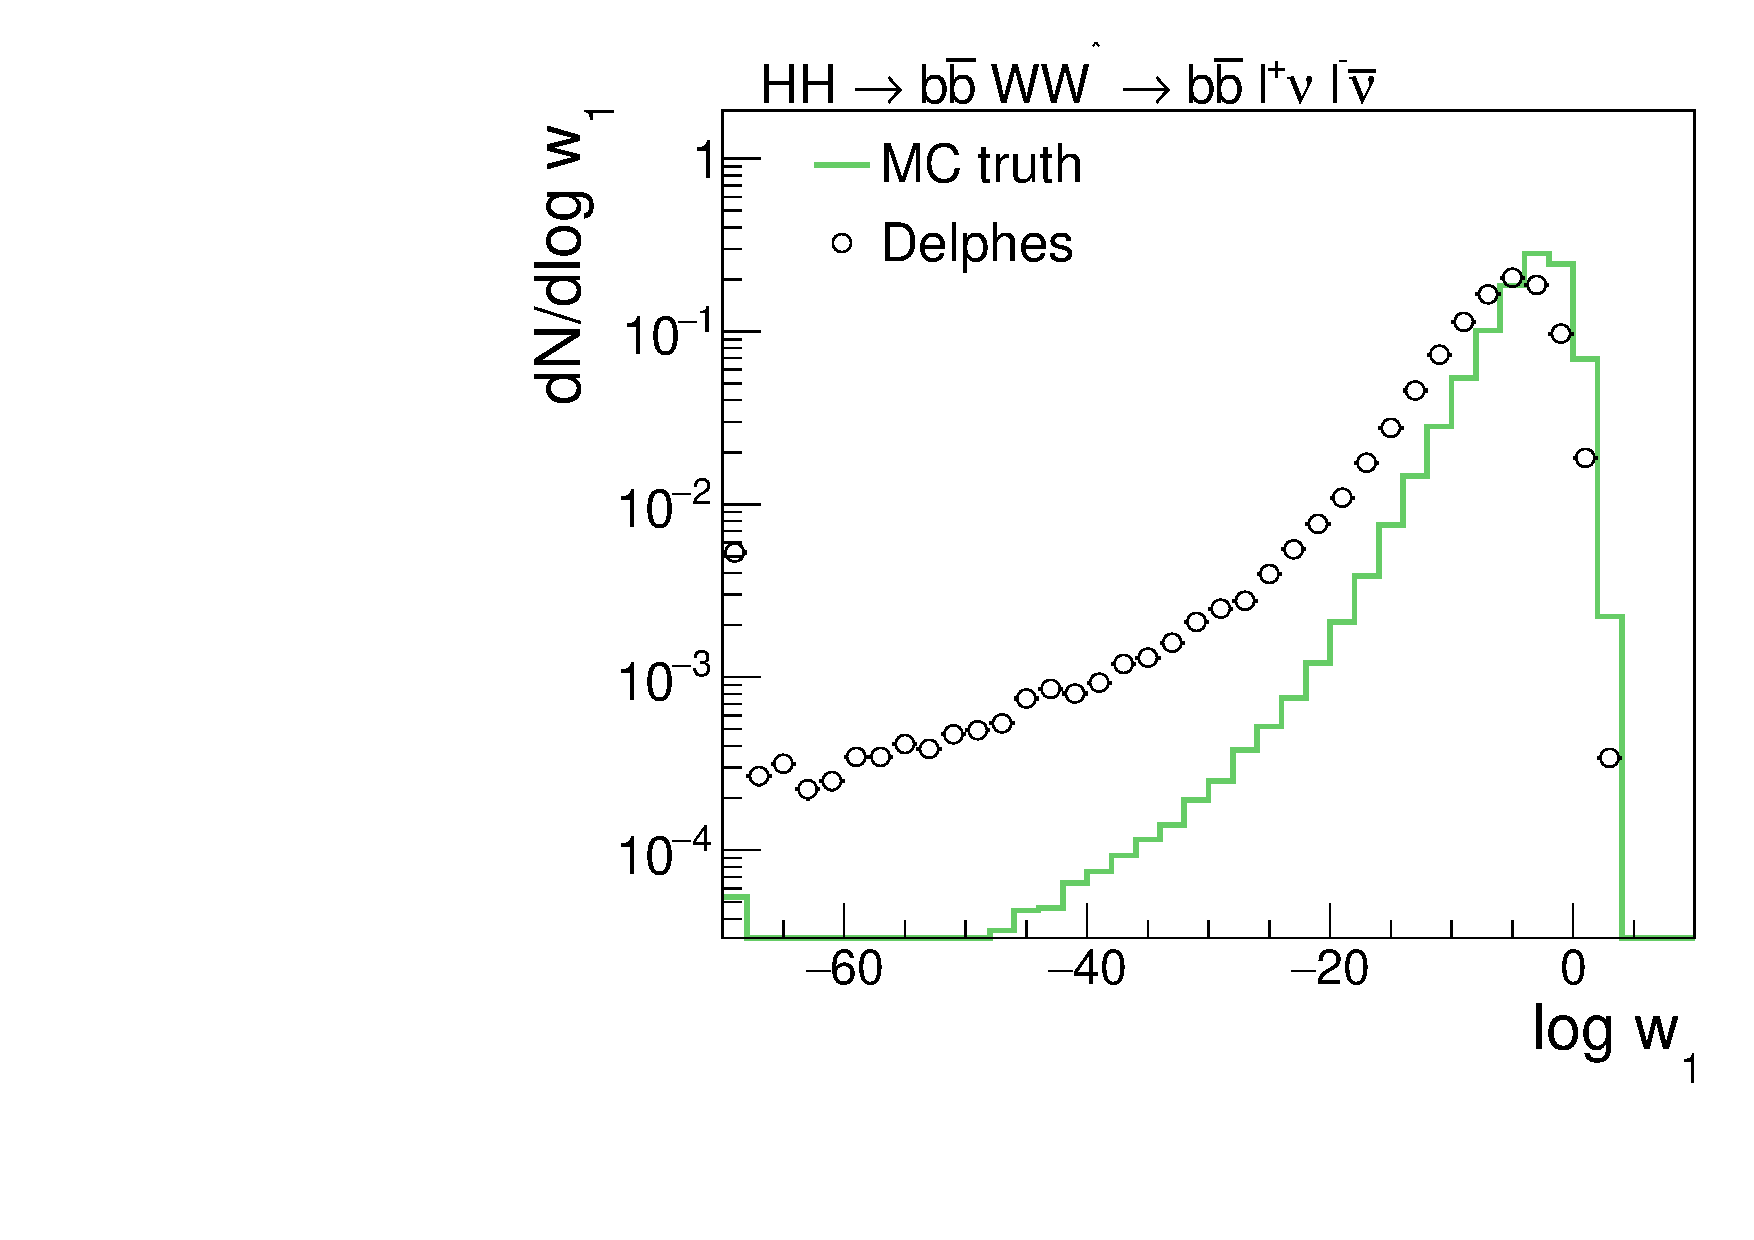
\includegraphics[width=0.48\textwidth]{plots/makePlotsForPaper_delphes_vs_mctruth_probB_background.pdf}
\fi
\caption{
  Distributions in the PDs $w_{0}(\vecy)$ (upper) and $w_{1}(\vecy)$ (lower), computed according to Eqs.~\ref{eq:mem_signal} and~\ref{eq:mem_background},
  for $\dihiggs$ signal (left) and $\ttbar$ background (right) events.
  The weights are computed at MC-truth and at detector level.
}
\label{fig:probS_and_probB}
\end{figure}

The corresponding distributions in the LR $P(\vecy)$, computed according to Eq.~\ref{eq:memLR}, are shown in Fig.~\ref{fig:memLR}.
Signal events are characterized by high values of $P(\vecy)$, while background events typically have low values.
The secondary peak of the distribution at low values for $\dihiggs$ signal (at high values for $\ttbar$ background) events
is due to events in which the event kinematics are atypical for signal (background) events, 
resulting in the PD for the wrong hypothesis $w_{1}(\vecy)$ ($w_{0}(\vecy)$) to be higher than the PD for the correct hypothesis $w_{0}(\vecy)$ ($w_{1}(\vecy)$).
About $X\%$ of signal ($X\%$ of background) events populate the secondary peak in case the LR $P(\vecy)$ is computed at MC-truth level.
The fraction of $\dihiggs$ signal ($\ttbar$ background) events that populate the secondary peak increases to $X\%$ ($X\%$) in case the LR $P(\vecy)$ is computed at detector level.
The ``receiver-operating-characteristic'' (ROC) curves~\cite{ROCcurve} that correspond to these distributions are shown in Fig.~\ref{fig:ROC}.
The ROC curve quantifies the separation between the $\dihiggs$ signal and the $\ttbar$ background
and is obtained by varying the threshold of a cut on the LR $P(\vecy)$ and plotting the fractions of signal and background events passing the cut.
For a signal efficiency of $35\%$, the $\ttbar$ background is reduced by almost three orders of magnitude, to a level of $1.2$ permille, in case the LR $P(\vecy)$ is computed at MC-truth level.
In case the LR $P(\vecy)$ is computed at detector level, the $\ttbar$ background is reduced to a level of $2.5$ permille.
The main reason for the degradation in separating the $\dihiggs$ signal from the $\ttbar$ background that occurs at detector level
are signal events in which one of the bottom quarks originating from the $\PHiggs$ boson decay is not reconstructed as $\Pbottom$-jet at detector level
and a light quark or gluon jet is misidentified as $\Pbottom$-jet instead.
If this happens, the mass of the two detector-level jets that are reconstructed as $\Pbottom$-jets are often incompatible with $m_{\PHiggs}$.
To better gauge the separation of the $\dihiggs$ signal from the $\ttbar$ background achieved by the LR $P(\vecy)$,
we compute signal efficiencies and background rates that one would obtain by cutting on the mass $\mbb$ of the $\Pbottom$-jet pair, shown in Fig.~\ref{fig:mbb}, for comparison.
Fitting the peak of the distribution in $\mbb$ obtained after the jet calibration is applied in $\dihiggs$ signal events
with a normal distribution yields a mean of $117.7$~\GeV and a standard deviation of $19.6$~\GeV.
Selecting events for which the mass $\mbb$ is within $1$ ($2$) standard deviations around the mean
keeps $68.9\%$ ($86.9\%$) of the $\dihiggs$ signal and $22.1\%$ ($40.6\%$) of the $\ttbar$ background.
The mass $\mbb$ is presumably one of the most powerful single observable to separate the $\dihiggs$ signal from the $\ttbar$ background.
The conclusion that we draw from the numbers quoted in this paragraph is that by exploiting the full difference in event kinematics between the $\dihiggs$ signal and the $\ttbar$ background with the MEM
one can significantly improve the separation of the $\dihiggs$ signal from the $\ttbar$ background compared to imposing simple cuts on single observables.
We remark that the misidentification of hadrons as leptons is not simulated in $\textsc{DELPHES}$ and hence not accounted for in the detector-level ROC curve shown in Fig.~\ref{fig:ROC}.
We expect this have only a small effect on the ROC curve,
as analysis of $\dihiggs$ production performed by the CMS collaboration in the decay channel $\Pbottom\APbottom\PW\PW\virt$ in LHC Run $2$
found the misidentification of hadrons as leptons to constitute only a small, if not negligible, source of background.

\begin{figure}
\ifx\ver\verPreprint
\setlength{\unitlength}{1mm}
\begin{center}
\begin{picture}(160,66)(0,0)
\put(-1.0, 0.0){\mbox{\includegraphics*[height=66mm]
 {plots/makePlotsForPaper_delphes_vs_mctruth_memLR_signal.pdf}}}
\put(80.0, 0.0){\mbox{\includegraphics*[height=66mm]
 {plots/makePlotsForPaper_delphes_vs_mctruth_memLR_background.pdf}}}
\end{picture}
\end{center}
\fi
\ifx\ver\verPAPER
\centering
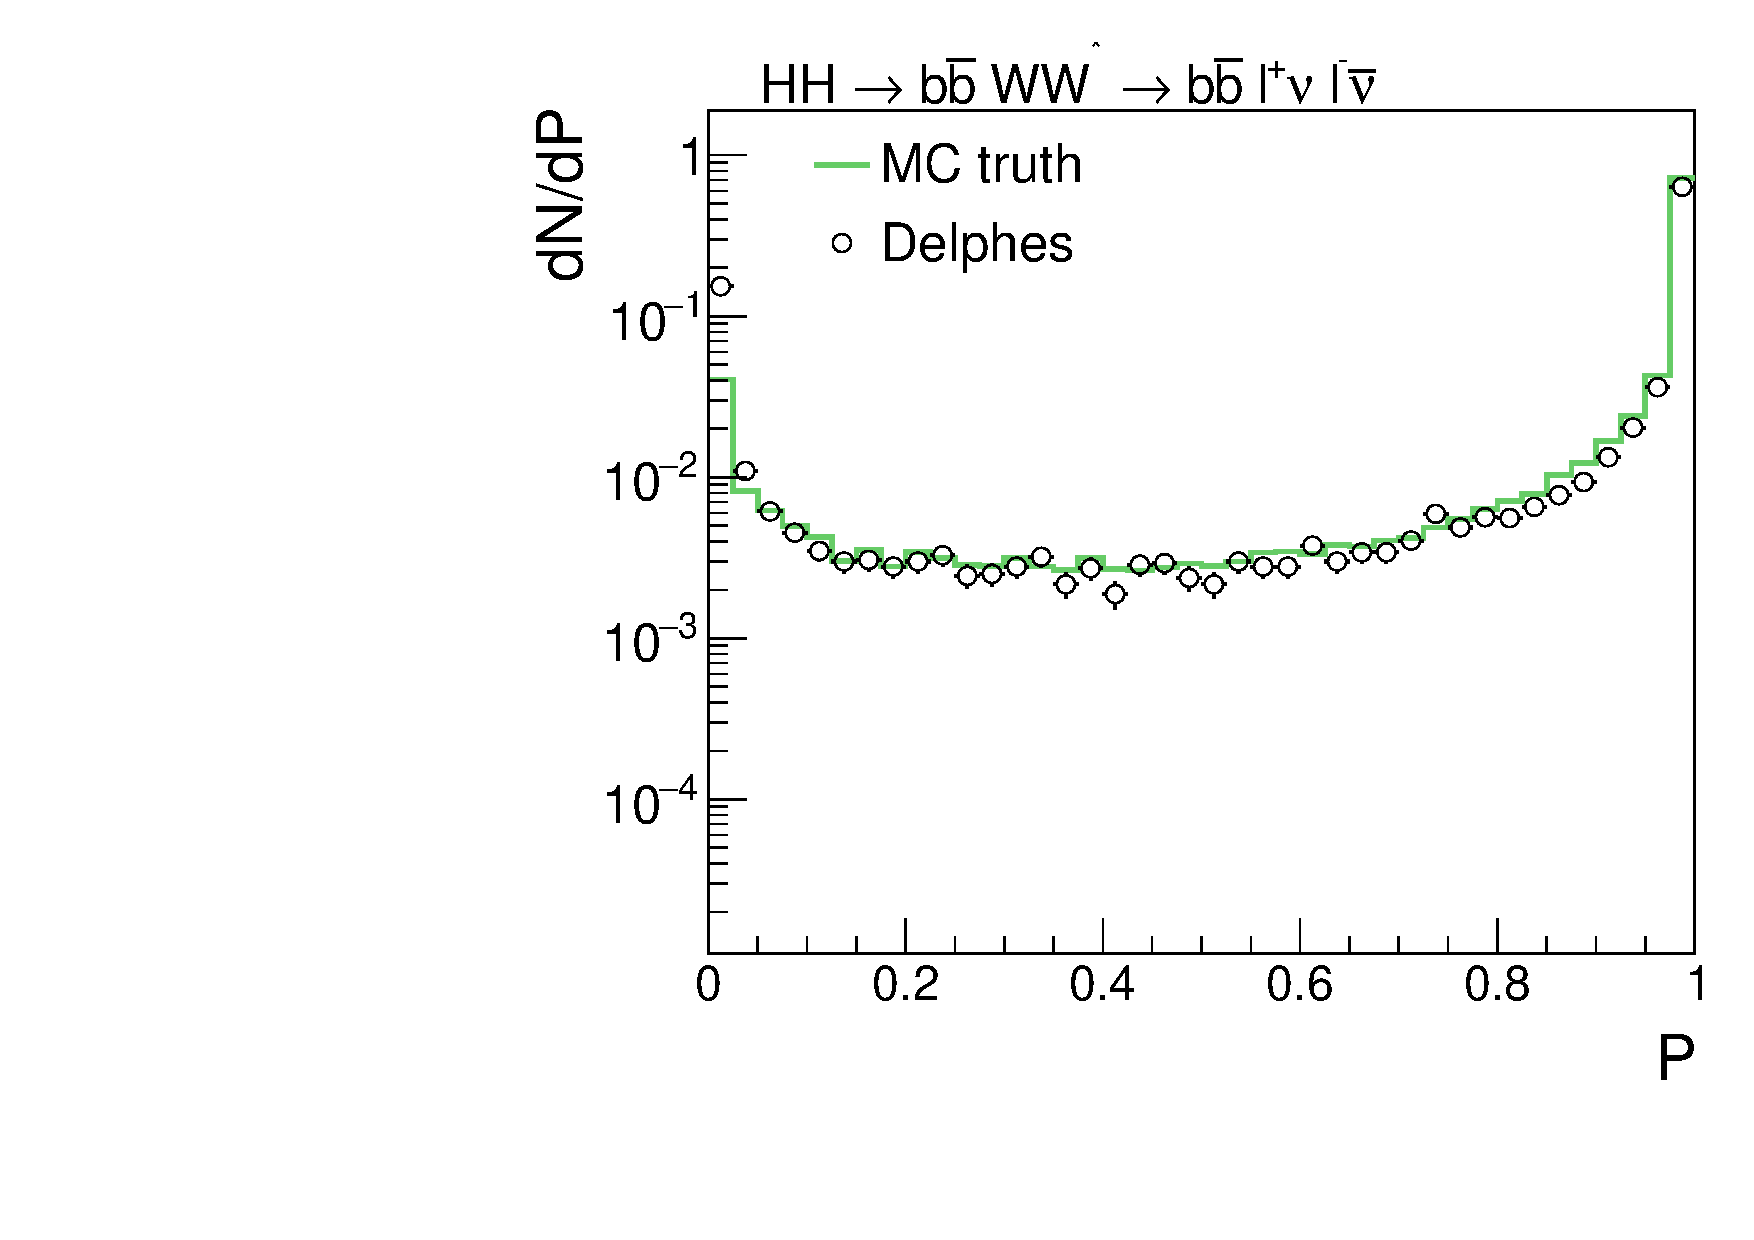
\includegraphics[width=0.48\textwidth]{plots/makePlotsForPaper_delphes_vs_mctruth_memLR_signal.pdf}
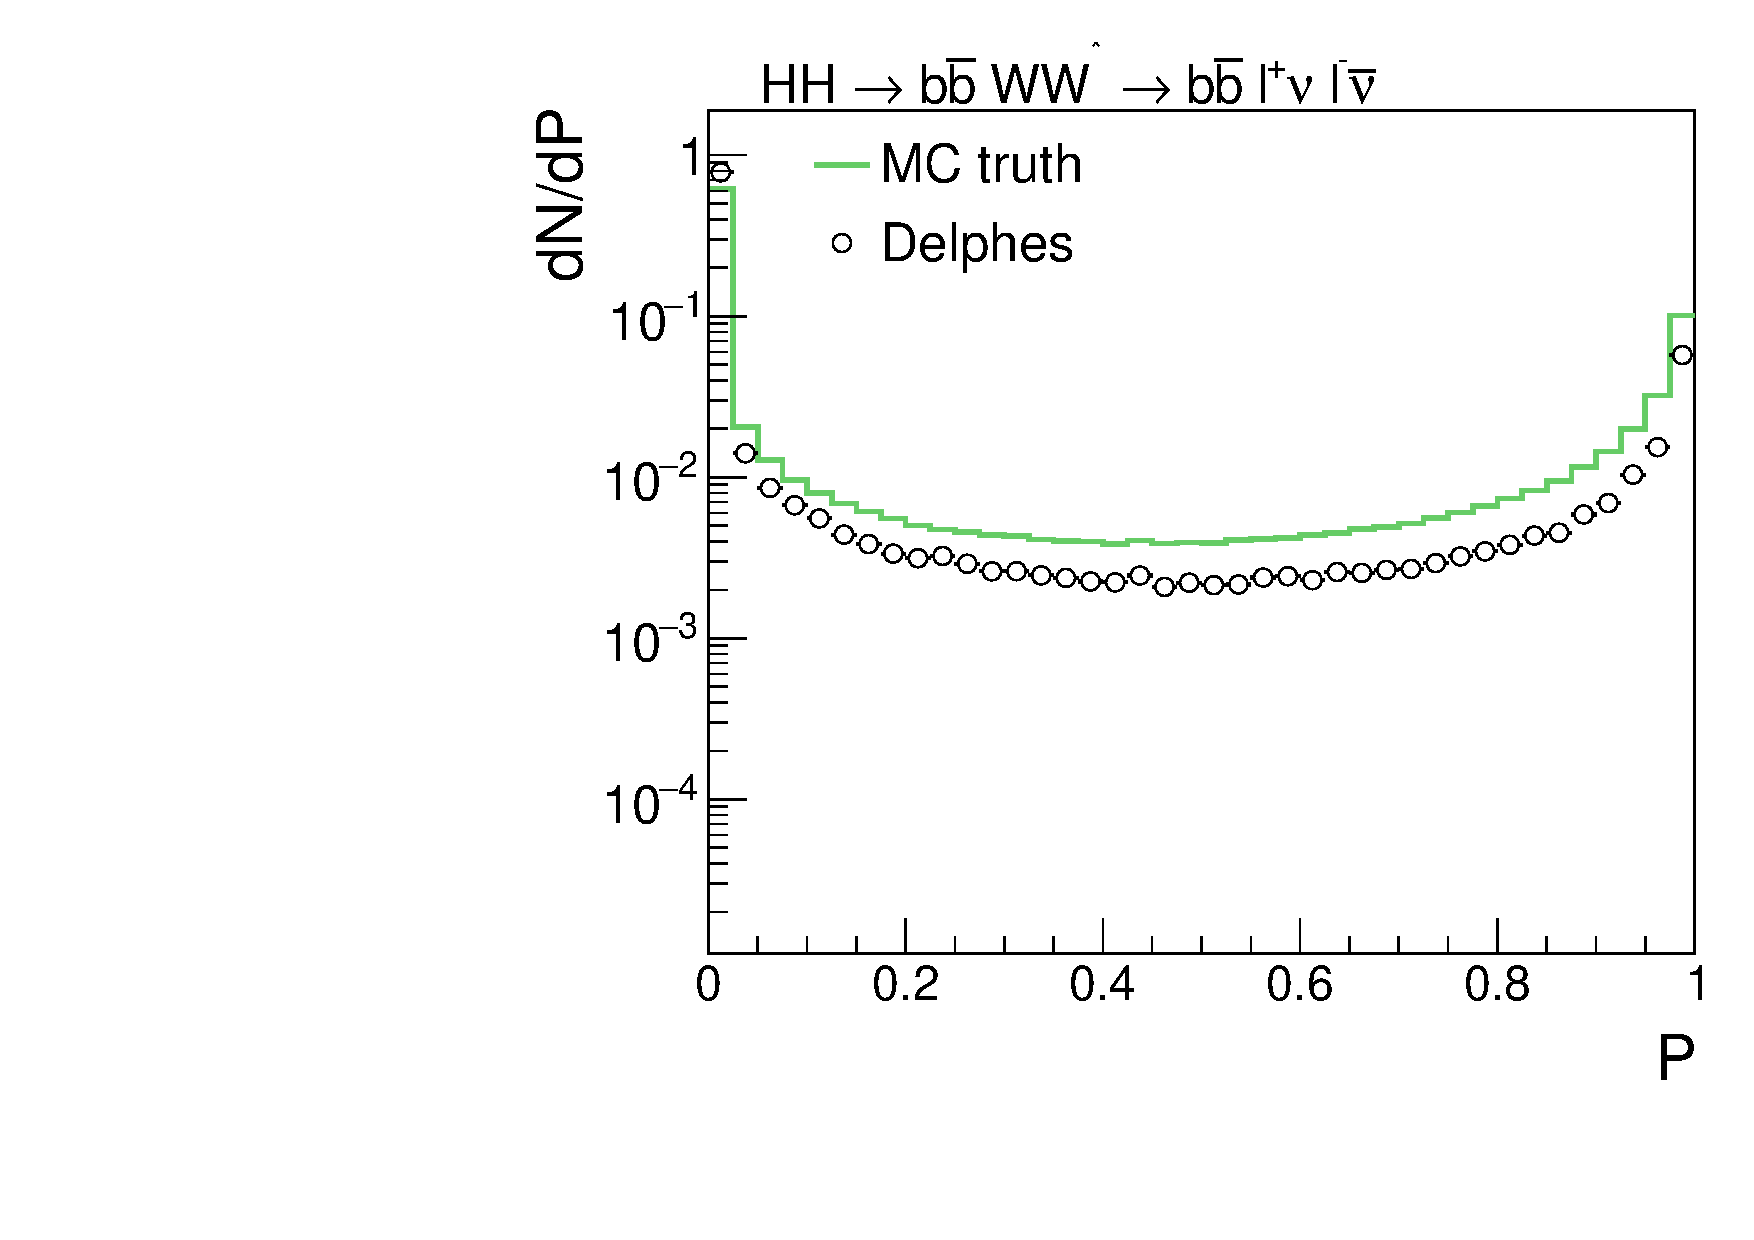
\includegraphics[width=0.48\textwidth]{plots/makePlotsForPaper_delphes_vs_mctruth_memLR_background.pdf}
\fi
\caption{
  Distributions in the LR $P(\vecy)$, computed according to Eq.~\ref{eq:memLR},
  for $\dihiggs$ signal (left) and $\ttbar$ background (right) events.
  The LR $P(\vecy)$ is computed using the PDs $w_{0}(\vecy)$ and $w_{1}(\vecy)$ shown in Fig.~\ref{fig:probS_and_probB} as input
  and is computed at MC-truth and at detector level.
}
\label{fig:memLR}
\end{figure}

\begin{figure}
\ifx\ver\verPreprint
\setlength{\unitlength}{1mm}
\begin{center}
\begin{picture}(160,78)(0,0)
\put(39.5, 0.0){\mbox{\includegraphics*[height=78mm]
 {plots/makePlotsForPaper_delphes_vs_mctruth_ROC.pdf}}}
\end{picture}
\end{center}
\fi
\ifx\ver\verPAPER
\centering
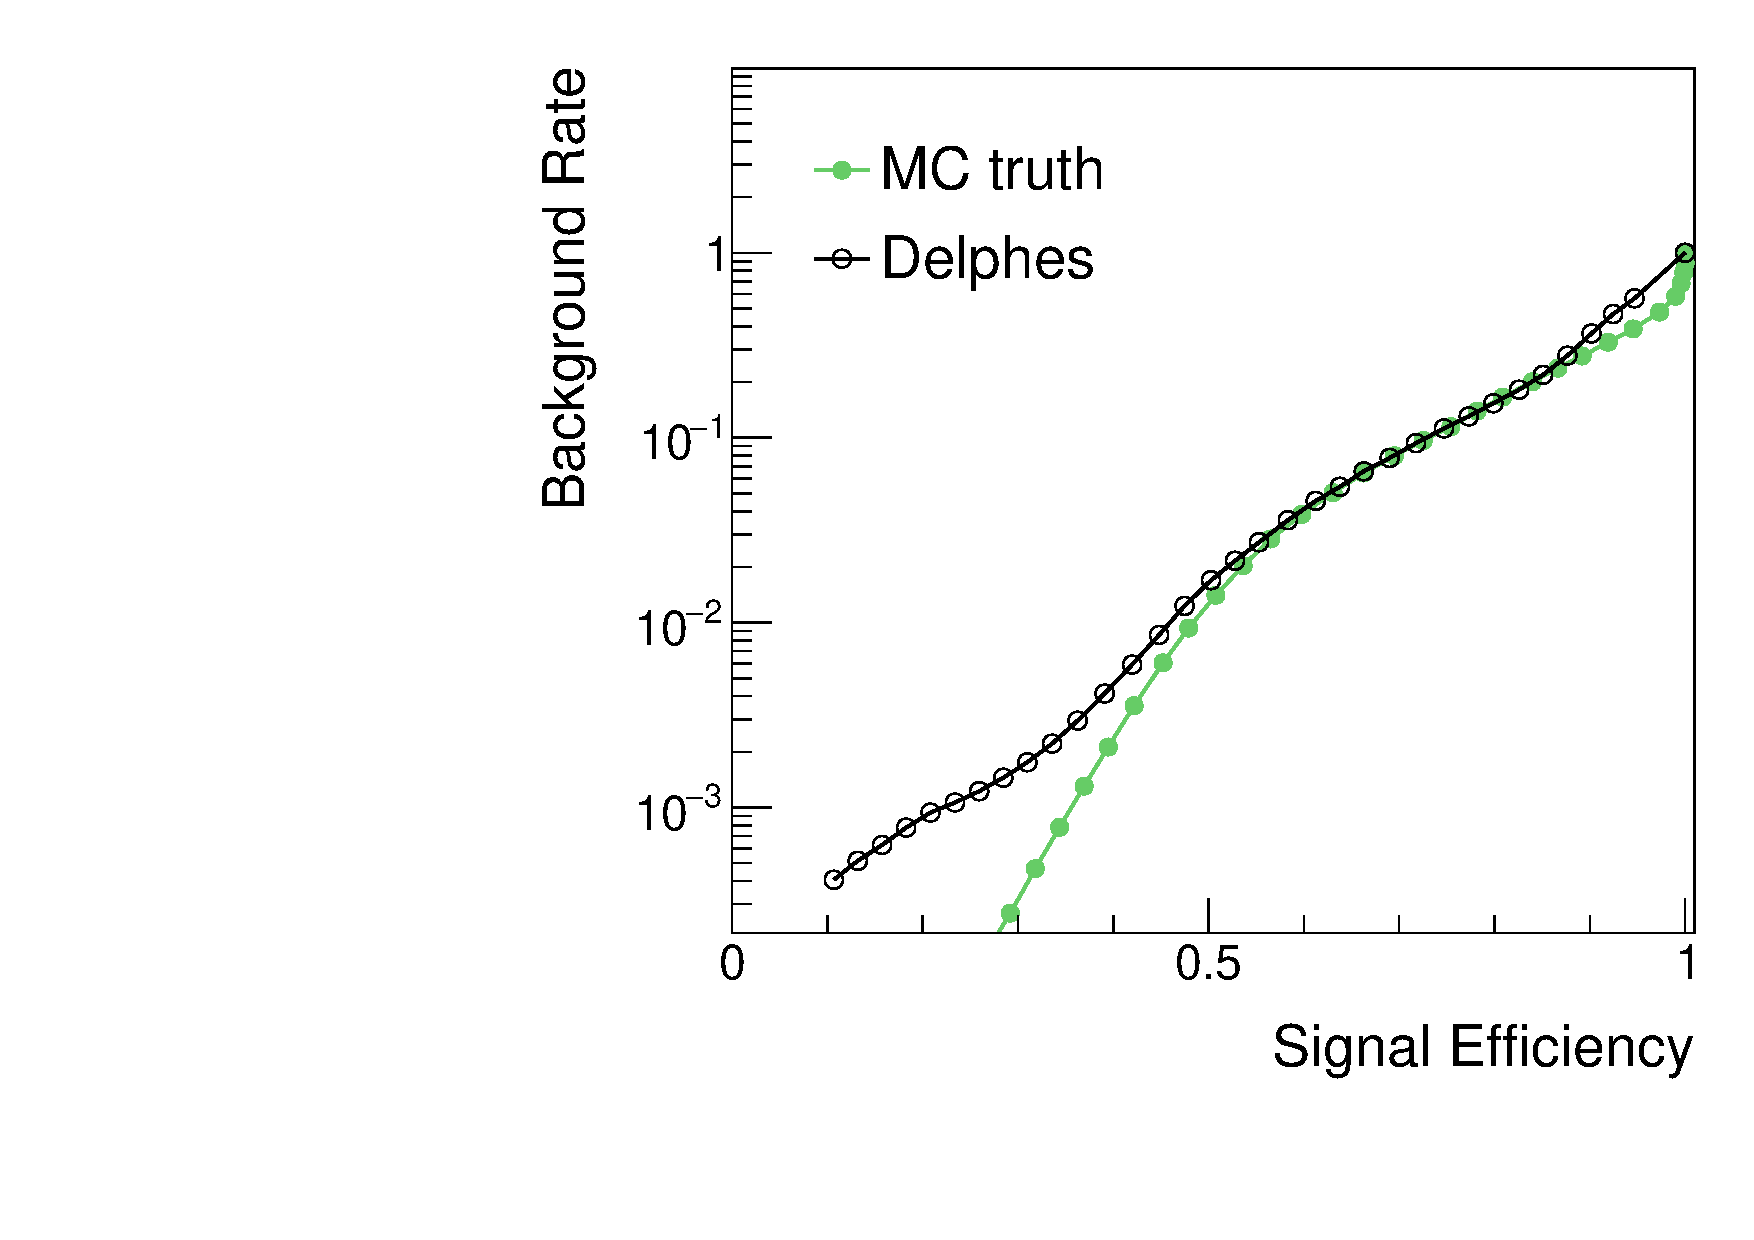
\includegraphics[width=0.48\textwidth]{plots/makePlotsForPaper_delphes_vs_mctruth_ROC.pdf}
\fi
\caption{
  Graphs of background rate versus signal efficiency (``ROC curve''), at MC-truth and at detector level,
  obtained by applying a cut on the distributions in the LRs $P(\vecy)$ shown in Fig.~\ref{fig:memLR}.
}
\label{fig:ROC}
\end{figure}

We conclude this section with a discussion of LO vs NLO...
